\section{Introduction}
\subsection{\mybox Définition}
\subsection{\mybox Machine Learninig}
\subsection{\mybox Deep Learning}
\subsection{\mybox Des applications}
\subsection{\mybox Experts  vs IA}

\begin{frame}{Introduction}
    \begin{enumerate}[<+-|alert@+>]
        \myitem
        L'intelligence artificielle est partout, mais elle trouve plus particulièrement
        des applications intéressantes dans le domaine de la santé.

        \myitem
        Les données médicales constituent une ressource inestimable pour prédire des maladies,
        diagnostiquer une pathologie ou améliorer le suivi des patients.

        \myitem
        L'\textbf{IA} est capable de poser un diagnostic fiable ou de lever des soupçons sur des
        pathologies.\mybox
    \end{enumerate}
\end{frame}




\begin{frame}{Définition}
    \begin{itemize}[<+-|alert@+>]
        \myitem
        Les algorithmes de \textbf{IA} est basé sur  l'injections des milliards de données
        dans un programme d'apprentissage,

        \myitem
        dans le cas des algorithmes du médecine, on apprend à ``reconnaître'' les signes
        de la maladie.\mybox
    \end{itemize}
    \only<1->{
        \centering
        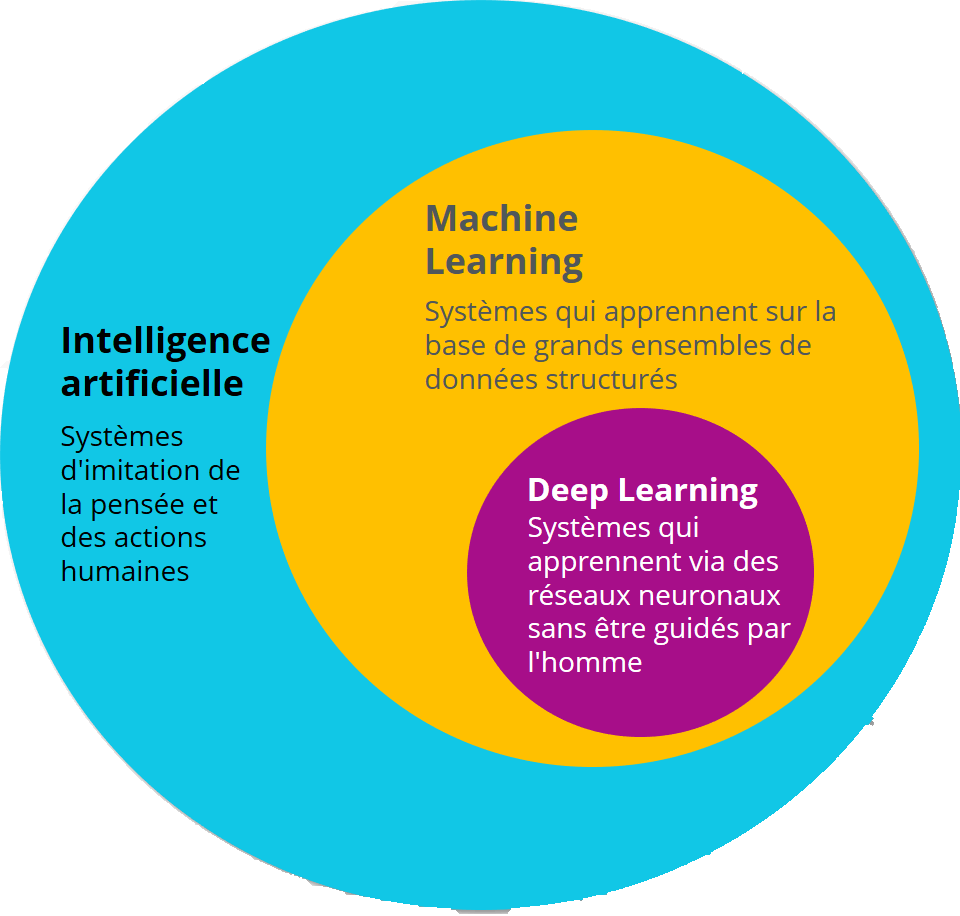
\includegraphics[height=0.3\textwidth,width=0.3\textwidth]{ai1a.png}
    }

\end{frame}

\begin{frame}{Machine Learninig}
    \begin{itemize}[<+-|alert@+>]
        \myitem
        ``Machine learninig'' apprentissage automatique, une méthode fondée sur
        la représentation mathématique et informatique de neurones
        biologiques, selon des modalités plus ou moins complexes.

        \myitem
        Les algorithmes d'apprentissage profond (deep learning) par exemple, dont
        l'usage explose depuis une dizaine d'années, font une analogie
        lointaine avec le fonctionnement cérébral en simulant un réseau de
        neurones organisés en différentes couches, échangeant les uns avec les
        autres.

        \myitem
        La force de cette approche est que l'algorithme apprend la
        tâche qui lui a été assignée par ``essais et erreurs''.\mybox
    \end{itemize}

    \only<1>{
        \vspace{-30mm}
        \centering
        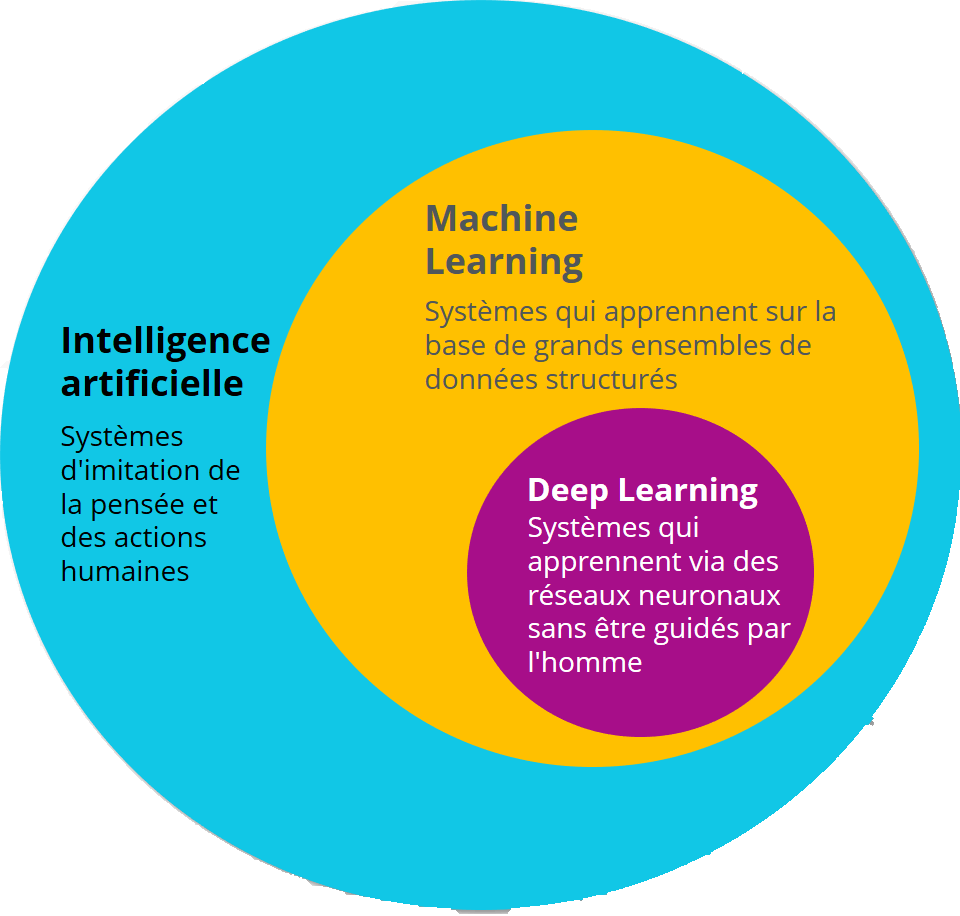
\includegraphics[height=0.4\textwidth,width=0.4\textwidth]{ai1a.png}
    }
    \vspace{80mm}

\end{frame}

\begin{frame}{Deep Learning}
    Utilisation des algorithmes d'intelligence artificielle pour permettre
    en quelque sorte aux ordinateurs d'apprendre par eux-mêmes On
    appelle cela l'apprentissage profond ou ``deep learning'' en anglais''.\mybox
    \\
    \bigskip
    \bigskip
    \centering
    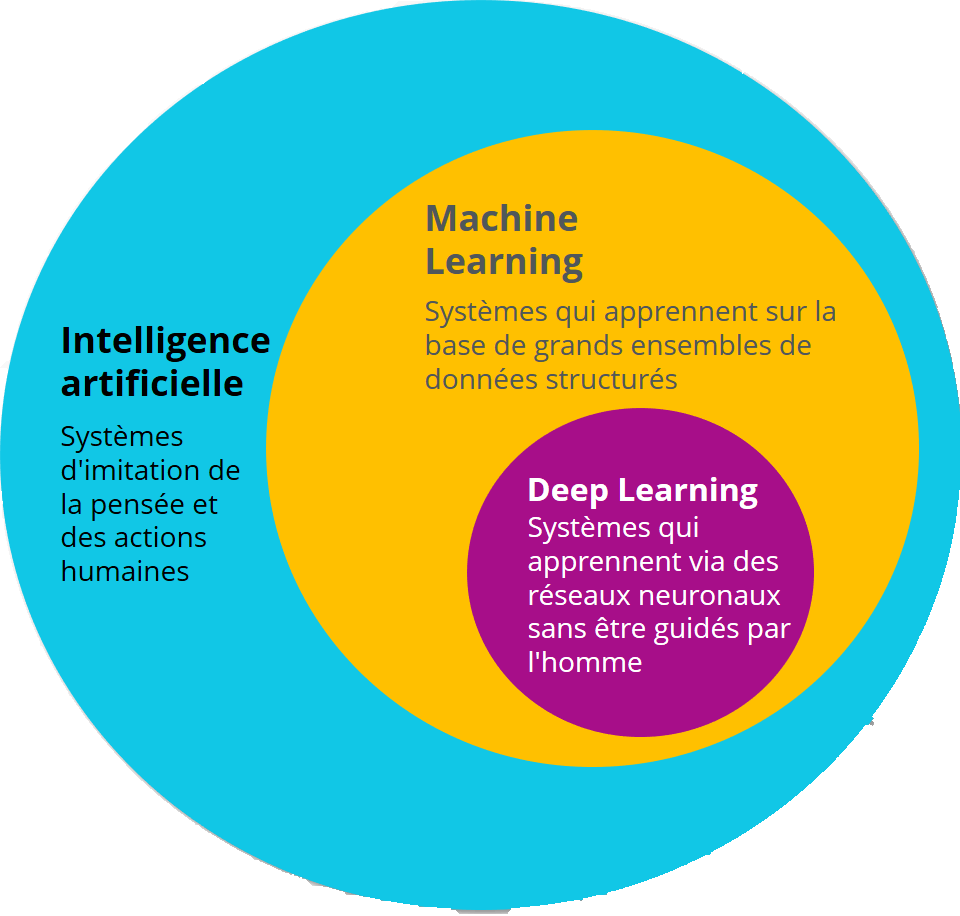
\includegraphics[height=0.3\textwidth,width=0.3\textwidth]{ai1a.png}
\end{frame}

\begin{frame}{Des applications}
    \begin{enumerate}[<+-|alert@+>]
        \myitem
        l'application de \textbf{IA} en traitement d'images, par exemple pour repérer de
        possibles mélanomes sur les photos de peau, ou bien pour dépister des
        rétinopathies diabétiques sur des images de rétines. Leur mise au point
        nécessite de grands échantillons d'apprentissage.
        \myitem
        en prend plus de 50 000 images dans le cas des mélanomes, et 128 000
        dans celui des rétinopathies, ont été nécessaires pour entraîner
        l'algorithme à identifier les signes de pathologies. Pour chacune
        de ces images on lui indique si elle présente ou non des signes
        pathologiques.
        \myitem
        A la fin de l'apprentissage, l'algorithme arrive à
        reconnaître avec une excellente performance de nouvelles images
            présentant une anomalie. \mybox
    \end{enumerate}
\end{frame}


\begin{frame}{Experts  vs IA}
    \begin{enumerate}[]
        \item \only<1->{
            \begin{exampleblock}{Les experts:}
                les procédures interventionnelles demandent une dextérité
                manuelle et un sens commun pour s'adapter à des situations changeantes.
            \end{exampleblock}
            }

        \item \only<2>{
            \begin{exampleblock} {IA:}
                Le travail des médecins radiologistes comprend de nombreuses tâches,
                dont les plus rapides comme la détection d'une anomalie ou les plus
                répétitives comme les mesures se prêtent bien à l'automatisation.\mybox
            \end{exampleblock}
            }
            \vspace{80mm}
    \end{enumerate}
\end{frame}
